\titledquestion{Highway Speed-Limit Sign Schedule}

There is a highway of length $L$ kilometers from Alpha Town to Beta City and there are $n$ traffic signs along the highway. Each speed-limit sign $i$ at $x_i$ ($0=x_1<x_2<\cdots<x_n<L$) kilometers from the origin has a speed limit $v_i$, indicating that you can travel at a speed of at most $v_i$ kilometers per hour until you reach the next sign or arrive at your destination. There is also a sign at Alpha Town ($x_1=0$) which sets the initial speed limit.

\begin{center}
	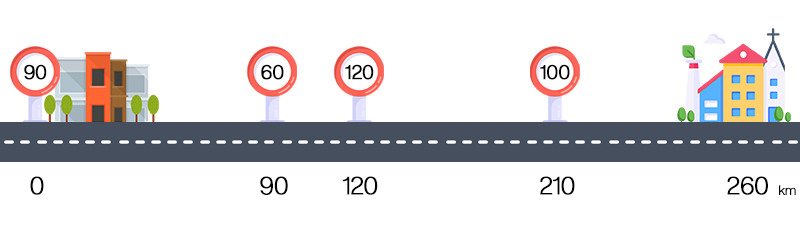
\includegraphics[width = \linewidth]{img/highway.png}
\end{center}

For example, assume we have $n=4$ and $L=260$ as the figure shown above. Then, it will take at least $\frac{90-0}{90}+\frac{120-90}{60}+\frac{210-120}{120}+\frac{260-210}{100}=2.75$ hours to travel from Alpha Town to Beta City under these speed limits.

In order to improve the traffic efficiency, the highway administration department decides to remove some speed-limit signs along the highway. However, due to the traffic restrictions of Alpha Town, the first sign at the origin $x_1=0$ cannot be removed.

Please come up with a dynamic programming algorithm to \textbf{minimize the travel time} from Alpha Town to Beta City by removing no more than $K$ speed-limit signs.

\vspace{0.2in}

\begin{parts}
	\part[2] Define your subproblem for this question.
	\begin{solution}
		%%%%%%%%%%%%%%%%%%%%%%%%%%%%%%%%%%%%%%%%%%%%%%%%%%
		%  Replace the `vspace{2.0in}' with your answer.  
		%%%%%%%%%%%%%%%%%%%%%%%%%%%%%%%%%%%%%%%%%%%%%%%%%%
		% \vspace{2.0in}
		\\let $dp[i][j]$ be the minimal time we will take from $x_1 = 0$ to the $x_i$,
		and the $i$-th sign is remained, $j$ speed-limit signs in the first $i$ signs are removed.\\
		% \\let $dp[i][j][k]$ be the minimal time we will remove some of the signs of $1,2,\cdots,i$,
		% and at most removed $j$ speed-limit signs,
		% and the consecutive $k$ signs are removed start from the $i$-th sign and to its forward.\\
	\end{solution}

    \newpage

	\part[5] Give your Bellman equation to solve the subproblems.
	\begin{solution}
		%%%%%%%%%%%%%%%%%%%%%%%%%%%%%%%%%%%%%%%%%%%%%%%%%%
		%  Replace the `vspace{3.0in}' with your answer.  
		%%%%%%%%%%%%%%%%%%%%%%%%%%%%%%%%%%%%%%%%%%%%%%%%%%
		% \vspace{3.0in}
		\\let $x_{n+1}=L$\\
		$1\leq i\leq n+1; j < i;  j\leq K$\\\\
		$dp[i][j]=min\{dp[k][j-(i-k-1)]+\frac{x_i-x_k}{v_k}\},k=(i-j-1),\cdots,i-1$\\
		% $dp[i][j][0]=min\{dp[i-1][j][k]+\frac{x_{i+1}-x_{i}}{v_{i}}\}$$,(k\leq j)$\\
		% $dp[i][j][k]=min\{dp[i-1][j-1][k-1]+\frac{x_{i+1}-x_{i}}{v_{i-k+1}}\}$$,(1\leq k\leq j)$\\
		\paragraph{Explanation:}
		\begin{itemize}
			% \item if $k\neq 0$,it means that the we will remove the $(i-k+1),\cdots,i$-th signs, 
			% \item if $k=0$, it means that 
			
			%$i$-th sign is not removed. So the following interval will at the speed of $v_i$.
			% \item the following line means that we will remove the $i$-th sign. Since it is consecutive $k$ signs are removed, so the following interval will at the speed of before, i.e. $v_{i-k+1}$.
			% \item $dp[i][j][0]$ means that the $i$-th sign is not removed. So the following interval will at the speed of $v_i$.
			% \item the following line means that we will remove the $i$-th sign. Since it is consecutive $k$ signs are removed, so the following interval will at the speed of before, i.e. $v_{i−k+1}$.
			\item since the $i$-th sign is not removed, so $j<i$.
			\item $k$ means that from the $k+1$-th sign to the $i-1$-th sign are all removed, and the $k$-th sign and the $i$-th sign are remained,
			so there are totally $i-1-k$ signs are removed, so it should transform from $dp[k][j-(i-k-1)]$, and during the period of $x_k$ to $x_i$,
			the limit speed if $v_k$.
			\item since we removed $i-k-1$ signs this time, so $i-k-1\leq j$, $i.e. k\geq i-j-1$
			
		\end{itemize}
	\end{solution}

	\part[2] What is the answer to this question in terms of the subproblems?
	\begin{solution}
		%%%%%%%%%%%%%%%%%%%%%%%%%%%%%%%%%%%%%%%%%%%%%%%%%%
		%  Replace the `vspace{1.5in}' with your answer.  
		%%%%%%%%%%%%%%%%%%%%%%%%%%%%%%%%%%%%%%%%%%%%%%%%%%
		% \vspace{1.5in}
		% \\$min\{dp[n][K][i],i=0,1,\cdots,K\}$\\
		\\$min\{dp[n+1][i],i=0,1,\cdots,K\}$\\
	\end{solution}

	\part[1] What is the runtime complexity of your algorithm?
	\begin{solution}
		%%%%%%%%%%%%%%%%%%%%%%%%%%%%%%%%%%%%%%%%%%%%%%%%%%
		%  Replace the `vspace{1.0in}' with your answer.  
		%%%%%%%%%%%%%%%%%%%%%%%%%%%%%%%%%%%%%%%%%%%%%%%%%%
		% \vspace{1.0in}
		\\$\Theta(nk^2)$\\
	\end{solution}
\end{parts}